% File: jupiter-css-podc16-c1423.tex
% CSS state space of client c3 for the schedule of jupiter-schedule-podc16.tex

\documentclass{standalone}

% preamble for jupiter-paper related TikZ drawing
\usepackage{tikz}
\usetikzlibrary{shapes, positioning, arrows.meta, calc, backgrounds, fit}

% default horizontal/vertical distance
\def\hdist{1.8}
\def\vdist{1.8}

\newcommand{\state}[2]{% #1: state label; #2: position
  \node (#1) [circle, inner sep = 0pt, minimum size = 10mm, text width = 10mm, align = center, draw, #2, font = \Large] {$#1$};
}

\tikzset{every lower node part/.style = {red}}
\newcommand{\statesplit}[3]{% #1: state upper label; #2: state lower label; #3: position
  \node (#1) [circle split, draw, minimum size = 6mm, text width = 10mm, align = center, #3, font = \Large]
  {
	$#1$
	\nodepart{lower}
	$#2$
  };
}

\newcommand{\transition}[4][]{% #2: start state; #3: end state; #4: transition label; #1: transition label position (optional)
  \draw[>=Stealth, ->] (#2) to node [rectangle, draw, above = 2pt, sloped, #1, font = \small] {#4} (#3);
}

\newcommand{\ins}[2]{$\textsc{Ins}(#1,#2)$}
\newcommand{\del}[2]{$\textsc{Del}(#1,#2)$}

\tikzset{node distance = \vdist and \hdist}
\tikzset{path/.style = {draw, rounded corners, ultra thick, #1}}

\begin{document}
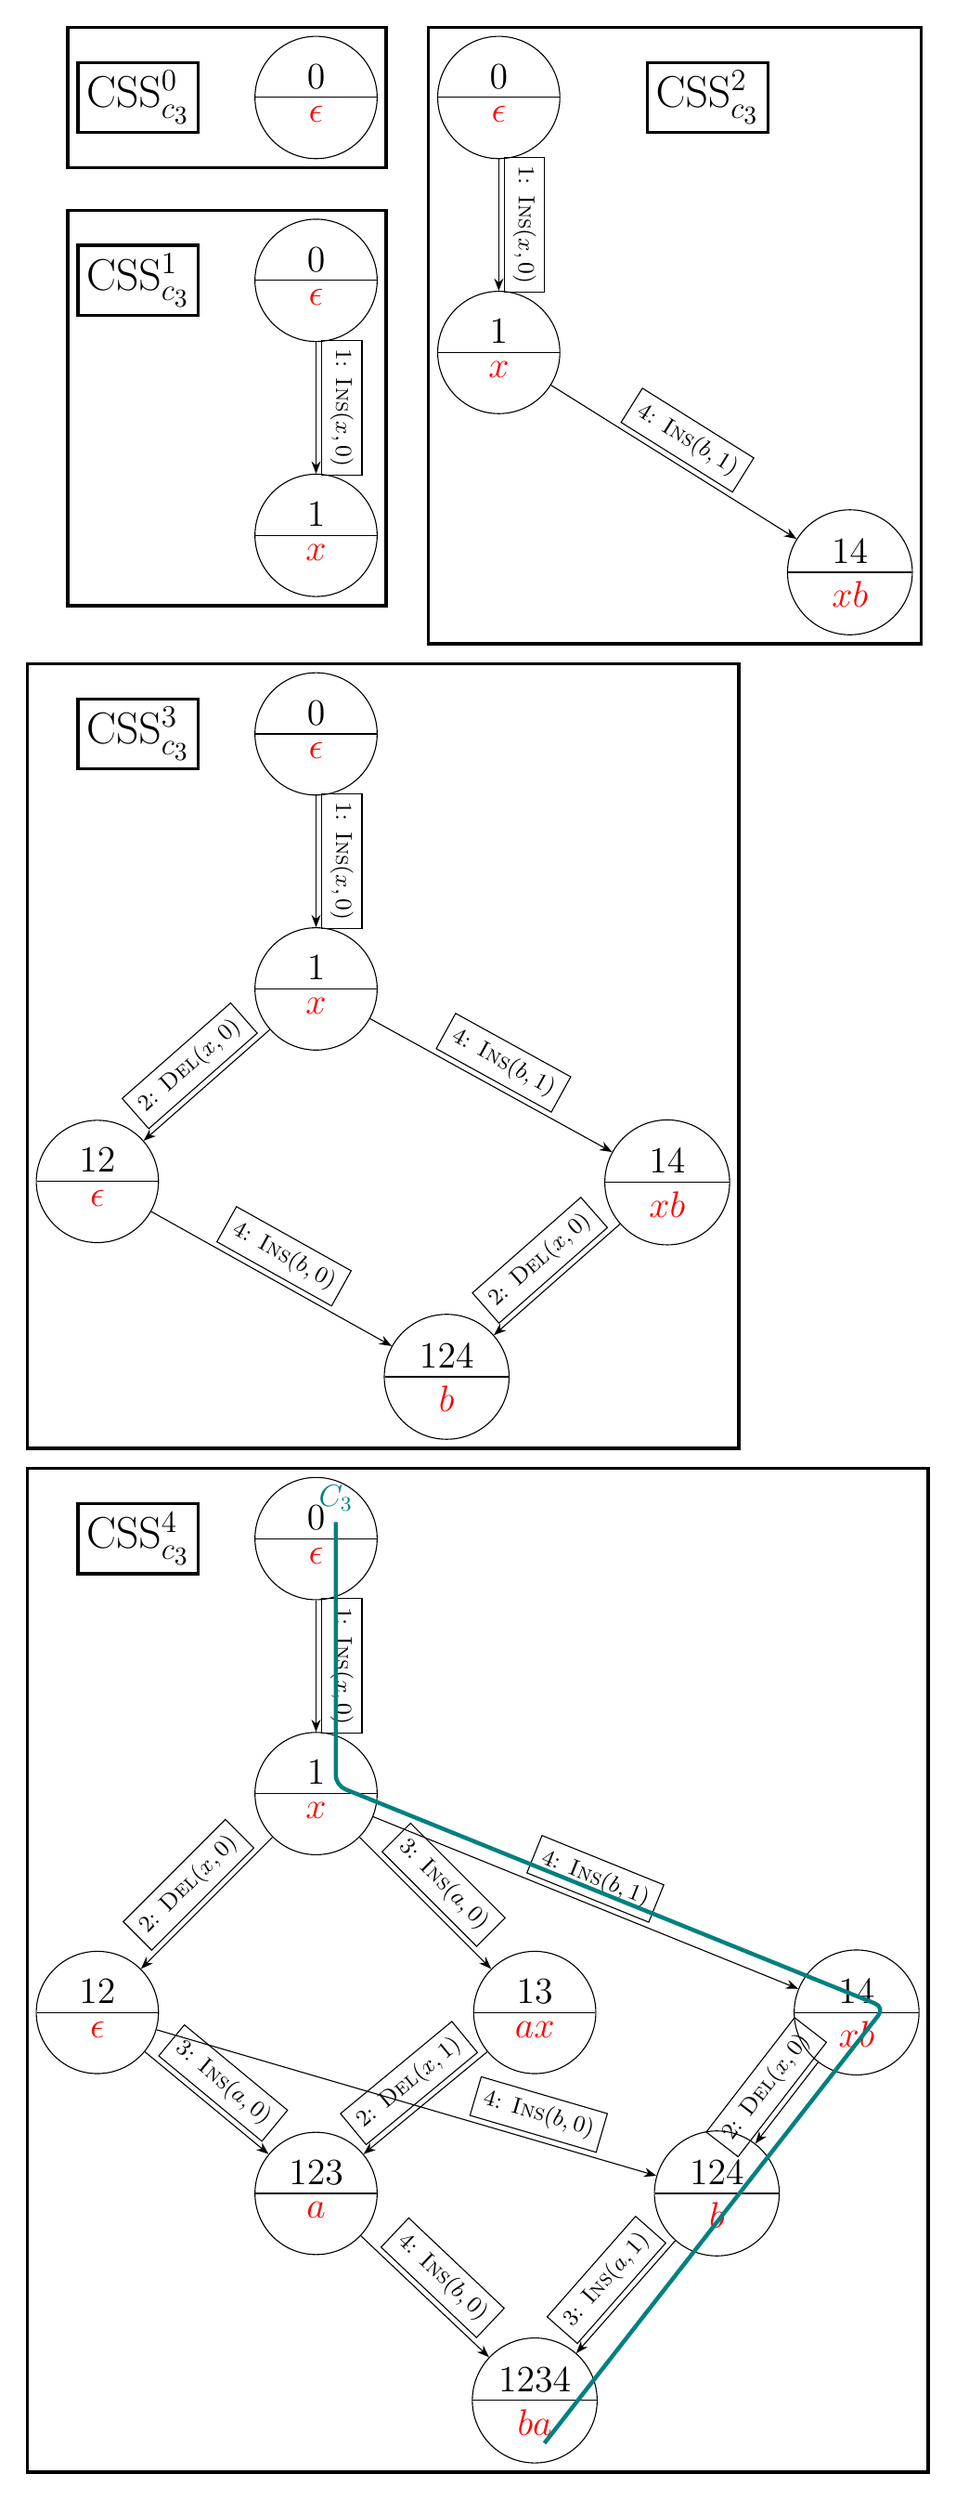
\begin{tikzpicture}[css/.style = {font = \LARGE, rectangle, draw, very thick},
	bg/.style = {rectangle, draw, very thick}]
  % init
  \begin{scope}
    \statesplit{0}{\epsilon}{}

    \begin{pgfonlayer}{background}
      \node (ss) [css, left = of 0.center, xshift = 6pt] {CSS$_{c_3}^{0}$};
      \node () [fit = (0) (ss), bg] {};
    \end{pgfonlayer}
  \end{scope}

  % 1st step: o1
  \begin{scope}[yshift = -2.5cm]
    \statesplit{0}{\epsilon}{}
    \statesplit{1}{x}{below = of 0}
    \transition{0}{1}{1: \ins{x}{0}}

    \begin{pgfonlayer}{background}
      \node (ss) [css, left = of 0.center, xshift = 6pt] {CSS$_{c_3}^{1}$};
      \node () [fit = (0) (1) (ss), bg] {};
    \end{pgfonlayer}
  \end{scope}

  % 2nd step: o1, o4
  \begin{scope}[xshift = 2.5cm]
    \statesplit{0}{\epsilon}{}
    \statesplit{1}{x}{below = of 0}
    \transition{0}{1}{1: \ins{x}{0}}
    % \statesplit{13}{ax}{below right = of 1}
    % \statesplit{14}{xb}{right = 1.5*\vdist of 13}
    \statesplit{14}{xb}{below right = \vdist and 2.0*\hdist of 1}
    \transition{1}{14}{4: \ins{b}{1}}

    \begin{pgfonlayer}{background}
      \node (ss) [css, right = of 0.center, xshift = 6pt] {CSS$_{c_3}^{2}$};
      \node () [fit = (0) (1) (14) (ss), bg] {};
    \end{pgfonlayer}
  \end{scope}

  % 3nd step: o1, o4, o2
  \begin{scope}[yshift = -8.7cm]
    \statesplit{0}{\epsilon}{}
    \statesplit{1}{x}{below = of 0}
    \transition{0}{1}{1: \ins{x}{0}}
    \statesplit{12}{\epsilon}{below left = 0.80*\vdist and \hdist of 1}
    \statesplit{14}{xb}{below right = 0.80*\vdist and 2.0*\hdist of 1}
    \transition{1}{14}{4: \ins{b}{1}}
    % \statesplit{13}{ax}{below right = of 1}
    % \statesplit{123}{a}{below = 2.1*\vdist of 1}
    \transition{1}{12}{2: \del{x}{0}}
    \statesplit{124}{b}{below left = 0.80*\vdist and \hdist of 14}
    \transition{14}{124}{2: \del{x}{0}}
    \transition[]{12}{124}{4: \ins{b}{0}}

    \begin{pgfonlayer}{background}
      \node (ss) [css, left = of 0.center, xshift = 6pt] {CSS$_{c_3}^{3}$};
      \node () [fit = (0) (1) (12) (14) (124) (ss), bg] {};
    \end{pgfonlayer}
  \end{scope}

  % 4th step: o1, o4, o2, o3
  \begin{scope}[yshift = -19.7cm]
    \statesplit{0}{\epsilon}{}
    \statesplit{1}{x}{below = of 0}
    \transition{0}{1}{1: \ins{x}{0}}
    \statesplit{12}{\epsilon}{below left = of 1}
    \statesplit{13}{ax}{below right = of 1}
    \statesplit{123}{a}{below = 2.1*\vdist of 1}
    \transition{1}{12}{2: \del{x}{0}}
    \transition{1}{13}{3: \ins{a}{0}}
    \transition{12}{123}{3: \ins{a}{0}}
    \transition{13}{123}{2: \del{x}{1}}
    \statesplit{14}{xb}{right = 1.5*\vdist of 13}
    \transition{1}{14}{4: \ins{b}{1}}

    \statesplit{124}{b}{right = 2.1*\hdist of 123}
    \transition{14}{124}{2: \del{x}{0}}
    \transition[near end]{12}{124}{4: \ins{b}{0}}
    
    \statesplit{1234}{ba}{below = 2*\vdist of 13}
    \transition{124}{1234}{3: \ins{a}{1}}
    \transition{123}{1234}{4: \ins{b}{0}}

    \begin{pgfonlayer}{background}
      \node (ss) [css, left = of 0.center, xshift = 6pt] {CSS$_{c_3}^{4}$};
      \node () [fit = (0) (1) (12) (13) (123) (14) (124) (1234) (ss), bg] {};
    \end{pgfonlayer}

    \path[path = {teal}] ($(0.center) + (40:10pt)$) node[above, font = \large] (c3) {$C_3$} -- ++(-90:2.0*\vdist) -- ++(-22:4.5*\vdist) -- ++(-128:4.2*\vdist);
  \end{scope}
\end{tikzpicture}
\end{document}